\documentclass[11pt,letterpaper]{article}

\usepackage[utf8]{inputenc}
\usepackage[left=.5in,right=.5in,top=.5in,bottom=.5in]{geometry}
\usepackage{amsmath,amssymb,amsfonts}
\usepackage{graphicx}
\usepackage{multicol}
\usepackage{hyperref}

% Simple semantic environments that compile cleanly in both LaTeX and LaTeXML.
\newenvironment{solution}
  {\par\medskip\noindent\textbf{Solution.}\par\smallskip}
  {\par\medskip}

\newenvironment{keyidea}
  {\par\medskip\noindent\textbf{Key Idea.}\par\smallskip}
  {\par\medskip}

\begin{document}

\begin{center}
{\Large Math 252: Section 10.2 --- Parametric Equations}\\
{\large Instructor Version}
\end{center}

\begin{enumerate}

\item \textbf{Motivation.}
Suppose a ball is thrown so that its path is described by
\[
y=-\frac{x^2}{72}+x,
\]
where \(x\) is the horizontal distance traveled and \(y\) is the height of the ball.

\begin{enumerate}
\item What information does this Cartesian equation tell us?

\begin{center}
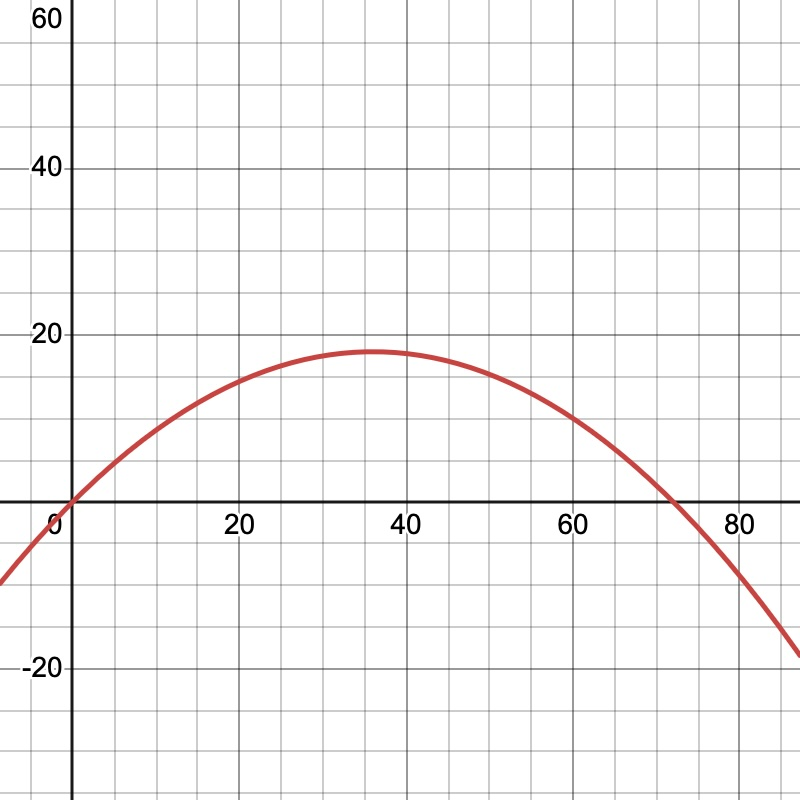
\includegraphics[scale=.25]{10_2_mot}
\end{center}

\begin{solution}
The equation gives the geometric path of the ball. It is a downward-opening parabola.

Factoring,
\[
y=x\left(1-\frac{x}{72}\right),
\]
shows that the \(x\)-intercepts are \(x=0\) and \(x=72\). Thus, if the ball begins and ends at ground level, its horizontal range is \(72\) feet.

The vertex occurs at
\[
x=-\frac{b}{2a}
=-\frac{1}{2(-1/72)}
=36.
\]
Then
\[
y(36)=-\frac{36^2}{72}+36=18.
\]
Thus the maximum height is \(18\) feet, attained after \(36\) horizontal feet.
\end{solution}

\item What important information does this equation not tell us?

\begin{solution}
It does not tell us how time is related to the motion. In particular, it does not specify the direction of travel, the position at a particular time, or how quickly the ball moves along the curve.
\end{solution}

\item Suppose instead that
\[
x=24\sqrt{2}\,t,
\qquad
y=-16t^2+24\sqrt{2}\,t,
\]
where \(t\) is measured in seconds. Why is this description more informative?

\begin{solution}
The parameter \(t\) gives the ball's position at each time. It also determines the direction of motion: as \(t\) increases, \(x\) increases, so the ball moves from left to right.

The ball returns to ground level when
\[
-16t^2+24\sqrt{2}\,t=0,
\]
so
\[
t(-16t+24\sqrt{2})=0.
\]
Hence
\[
t=0
\quad\text{or}\quad
t=\frac{3\sqrt{2}}{2}.
\]
Thus the flight lasts \(\frac{3\sqrt{2}}{2}\) seconds.
\end{solution}

\item Verify that eliminating \(t\) produces the original Cartesian equation.

\begin{solution}
From
\[
x=24\sqrt{2}\,t,
\]
we obtain
\[
t=\frac{x}{24\sqrt{2}}.
\]
Substitute this into \(y\):
\[
y=-16\left(\frac{x}{24\sqrt{2}}\right)^2
  +24\sqrt{2}\left(\frac{x}{24\sqrt{2}}\right).
\]
Since
\[
\left(24\sqrt{2}\right)^2=1152,
\]
we get
\[
y=-\frac{16x^2}{1152}+x
  =-\frac{x^2}{72}+x.
\]
\end{solution}
\end{enumerate}

\item \textbf{Definition.}
Let \(f\) and \(g\) be continuous on an interval \(I\). The equations
\[
x=f(t),\qquad y=g(t)
\]
are called \textbf{parametric equations}, and \(t\) is called the \textbf{parameter}.
As \(t\) varies through \(I\), the point
\[
(x,y)=\bigl(f(t),g(t)\bigr)
\]
traces a \textbf{plane curve} \(C\).

\textbf{Remark.} A Cartesian equation describes only the \emph{shape} of a curve. A parametrization also specifies how the curve is traced, including its initial and terminal points, direction of motion, whether the curve is traced more than once, and the position of the particle for each value of the parameter.

\item \textbf{Sketching Parametric Curves.}

When sketching a parametric curve it is often helpful to
\begin{enumerate}
\item determine the interval for the parameter,
\item eliminate the parameter whenever possible,
\item determine the appropriate Cartesian domain,
\item identify the initial and terminal points,
\item determine the direction in which the curve is traced.
\end{enumerate}

\item \textbf{Example 1.}
Sketch
\[
x=t^2-4,\qquad y=\frac{t}{2},
\qquad -2\le t\le 3.
\]

\begin{solution}
A useful table is
\[
\begin{array}{c|ccccc}
t&-2&-1&0&1&3\\ \hline
x=t^2-4&0&-3&-4&-3&5\\
y=t/2&-1&-\frac12&0&\frac12&\frac32
\end{array}
\]

Since \(y=t/2\), we have
\[
t=2y.
\]
Substituting into \(x=t^2-4\) gives
\[
x=(2y)^2-4=4y^2-4.
\]
Thus the Cartesian equation is
\[
\boxed{x=4y^2-4}.
\]

Because
\[
-2\le t\le 3,
\]
we have
\[
-1\le y\le \frac32.
\]
Therefore only the portion of the right-opening parabola satisfying
\[
\boxed{-1\le y\le \frac32}
\]
is traced.

At \(t=-2\), the curve begins at
\[
(0,-1).
\]
As \(t\) increases to \(0\), it moves left and upward to the vertex
\[
(-4,0).
\]
It then moves right and upward, ending at
\[
\left(5,\frac32\right).
\]
\end{solution}

\begin{center}
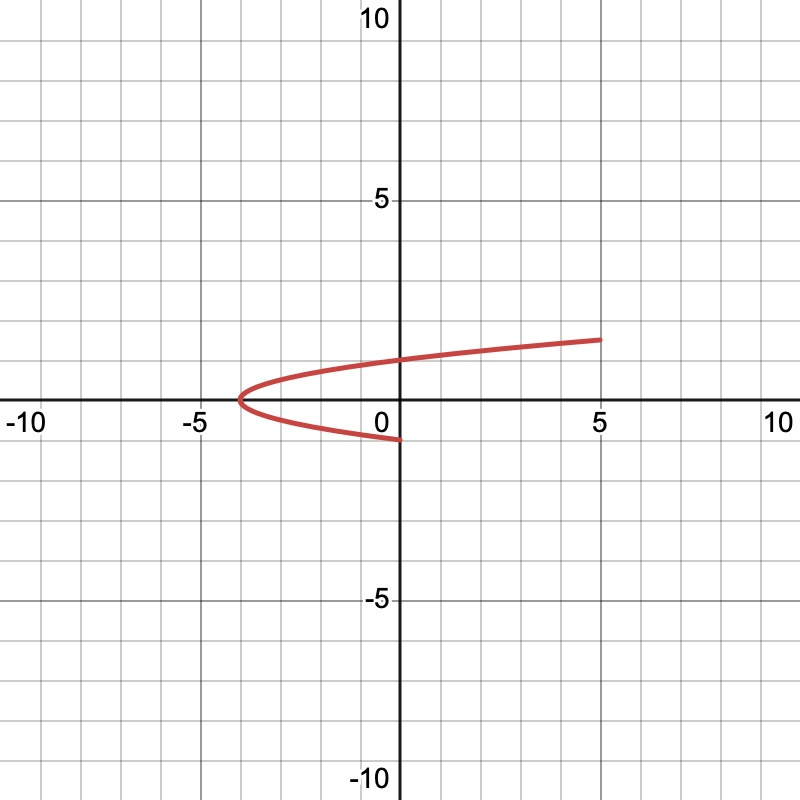
\includegraphics[scale=.3]{10_2_Ex1}
\end{center}

\item \textbf{Example 2.}
Sketch
\[
x=4t^2-4,\qquad y=t,
\qquad -1\le t\le \frac32.
\]

\begin{solution}
Since \(y=t\), substitution gives
\[
x=4y^2-4.
\]
Thus the curve lies on
\[
\boxed{x=4y^2-4}.
\]

The parameter interval gives
\[
\boxed{-1\le y\le \frac32}.
\]

The initial point is
\[
t=-1:\qquad (x,y)=(0,-1),
\]
and the terminal point is
\[
t=\frac32:\qquad
(x,y)=\left(4\left(\frac32\right)^2-4,\frac32\right)
=\left(5,\frac32\right).
\]

The curve moves from \((0,-1)\) left and upward to the vertex \((-4,0)\), then right and upward to \(\left(5,\frac32\right)\).
This is the same oriented curve as Example 1, even though the parametrizations are different.
\end{solution}

\begin{center}
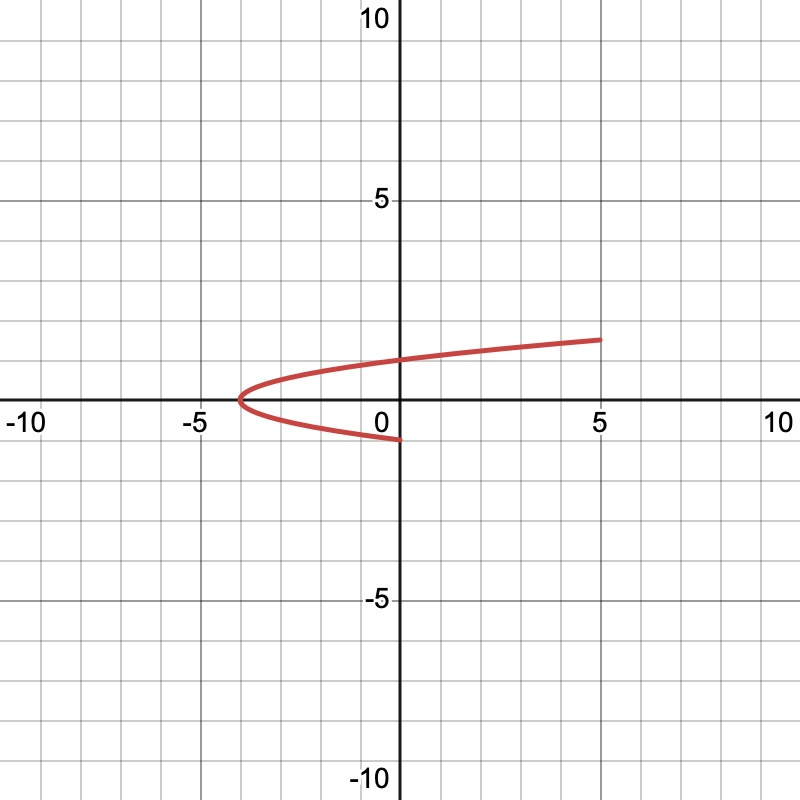
\includegraphics[scale=.3]{10_2_Ex1}
\end{center}


\item \textbf{Example 3.}
Sketch the curve by eliminating the parameter and finding the correct domain:
\[
x=\frac{1}{\sqrt{t+1}},
\qquad
y=\frac{t}{t+1},
\qquad t>-1.
\]

\begin{solution}
Rewrite \(y\):
\[
y=\frac{t}{t+1}
 =\frac{(t+1)-1}{t+1}
 =1-\frac{1}{t+1}.
\]
From
\[
x=\frac{1}{\sqrt{t+1}},
\]
we have
\[
x^2=\frac{1}{t+1}.
\]
Therefore
\[
\boxed{y=1-x^2}.
\]

The original parametrization imposes an important restriction. Since \(t>-1\),
\[
t+1>0,
\]
and
\[
x=\frac{1}{\sqrt{t+1}}>0.
\]
Hence the correct Cartesian domain is
\[
\boxed{x>0}.
\]

Thus the curve is the right-hand portion of the parabola
\[
y=1-x^2.
\]

For direction, as \(t\to-1^+\),
\[
x\to\infty,
\qquad
y=1-x^2\to-\infty.
\]
As \(t\to\infty\),
\[
x\to0^+,
\qquad
y\to1^-.
\]
Therefore the curve is traced from the lower right upward and to the left, approaching \((0,1)\) without reaching it.
\end{solution}

\begin{center}
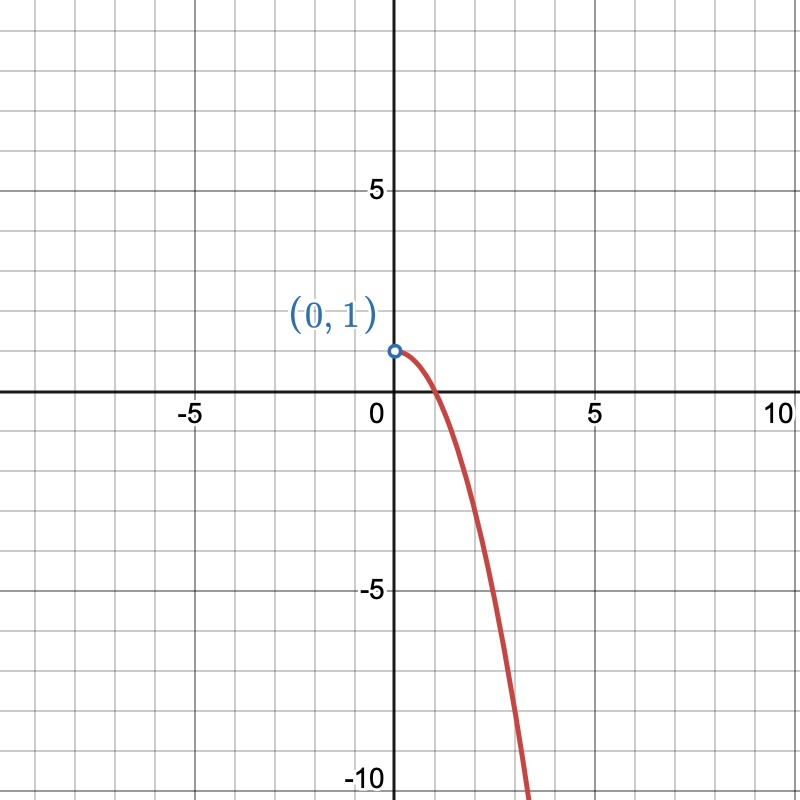
\includegraphics[scale=.3]{10_2_Ex3}
\end{center}

\item \textbf{Example 4.}
Sketch
\[
x=3\cos t,\qquad y=4\sin t,
\qquad 0\le t\le2\pi.
\]

\begin{solution}
Solve for the trigonometric expressions:
\[
\cos t=\frac{x}{3},
\qquad
\sin t=\frac{y}{4}.
\]
Using
\[
\cos^2t+\sin^2t=1,
\]
we obtain
\[
\boxed{\frac{x^2}{9}+\frac{y^2}{16}=1}.
\]
This is an ellipse centered at the origin with horizontal semiaxis \(3\) and vertical semiaxis \(4\).

Key points are
\[
\begin{array}{c|ccccc}
t&0&\frac{\pi}{2}&\pi&\frac{3\pi}{2}&2\pi\\ \hline
(x,y)&(3,0)&(0,4)&(-3,0)&(0,-4)&(3,0)
\end{array}
\]

The curve begins at \((3,0)\) and moves upward, so it is traced once in the counterclockwise direction.
\end{solution}

\begin{center}
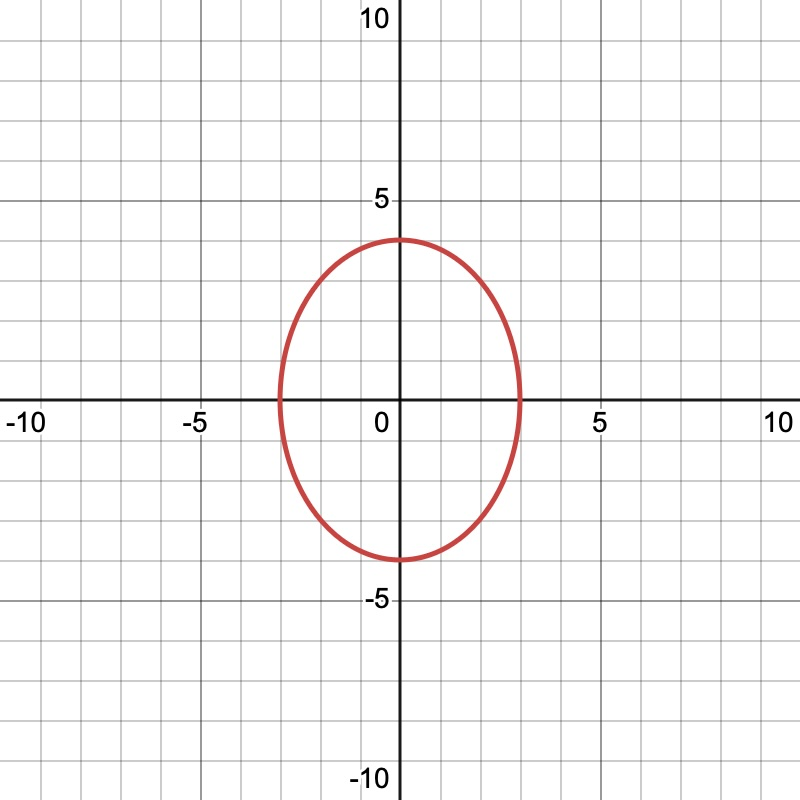
\includegraphics[scale=.3]{10_2_Ex4}
\end{center}


\item \textbf{Example 5.}
Sketch
\[
x=2\sin 2t,\qquad y=2\cos 2t,
\qquad 0\le t\le2\pi.
\]

\begin{solution}
We have
\[
\frac{x}{2}=\sin 2t,
\qquad
\frac{y}{2}=\cos 2t.
\]
Therefore
\[
\left(\frac{x}{2}\right)^2+
\left(\frac{y}{2}\right)^2=1,
\]
so
\[
\boxed{x^2+y^2=4}.
\]
This is a circle centered at the origin with radius \(2\).

At \(t=0\),
\[
(x,y)=(0,2).
\]
For small positive \(t\), \(x=2\sin 2t>0\), while \(y=2\cos 2t\) begins to decrease. Thus the point moves from the top of the circle toward the right, which is clockwise.

As \(t\) runs from \(0\) to \(2\pi\), the angle \(2t\) runs from \(0\) to \(4\pi\). Therefore the circle is traced twice, clockwise.
\end{solution}

\begin{center}
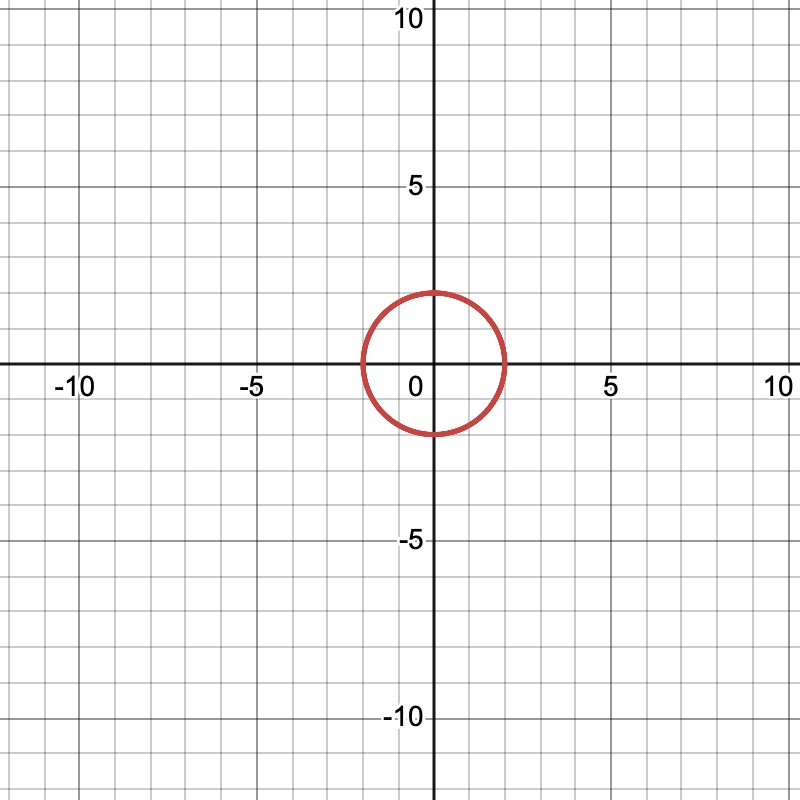
\includegraphics[scale=.3]{10_2_Ex5}
\end{center}

\item \textbf{Definition of a Smooth Curve.}
A curve \(C\), represented by
\[
x=f(t),\qquad y=g(t)
\]
on an interval \(I\), is called \textbf{smooth} if \(f'\) and \(g'\) are continuous on \(I\) and are not simultaneously zero, except possibly at the endpoints.

The curve is called \textbf{piecewise smooth} if the interval can be divided into finitely many subintervals on each of which the curve is smooth.

\begin{keyidea}
The vector
\[
\mathbf r'(t)=\bigl(f'(t),g'(t)\bigr)
\]
is the velocity vector of the parametrization. The condition
\[
\mathbf r'(t)\ne(0,0)
\]
ensures that the parametrization does not come to a complete stop at an interior point.
\end{keyidea}


\item \textbf{Example. Determining Whether a Curve is Smooth}

Decide whether each parametric curve is smooth.

\begin{enumerate}
\item \(x=t,\;y=t^2.\)

\begin{solution}
\[
x'(t)=1,\qquad y'(t)=2t.
\]
Since \(x'(t)\neq0\) for every \(t\), the derivatives are never simultaneously zero. Therefore the curve is smooth.
\end{solution}

\item \(x=t^3,\;y=t^2.\)

\begin{solution}
\[
x'(t)=3t^2,\qquad y'(t)=2t.
\]
Both derivatives are zero at \(t=0\). Hence the curve is \emph{not} smooth. This parametrization produces a cusp because the velocity vector is \((0,0)\) at \(t=0\).
\end{solution}
\end{enumerate}

\end{enumerate}

\end{document}
